%%%%%%%%%%%%%%%%%%%%%%%%%%
% document class: beamer %
%%%%%%%%%%%%%%%%%%%%%%%%%%
\documentclass{beamer}

%%%%%%%%%%%%
% PACKAGES %
%%%%%%%%%%%%
\usepackage{hyperref}
\usepackage{graphicx}
\usepackage{multirow}
\hypersetup{colorlinks=true,urlcolor=blue}


%%%%%%%%%%%%%%%%%%%%%%%%%%%%%
% no navigation bars please %
%%%%%%%%%%%%%%%%%%%%%%%%%%%%%
\setbeamertemplate{footline}[frame number]{}

%%%%%%%%%%%%%%%%%%%%%%%%%%%%%%%%
% no navigation symbols please %
%%%%%%%%%%%%%%%%%%%%%%%%%%%%%%%%
\setbeamertemplate{navigation symbols}{}

%%%%%%%%%%%%%%%%%%%%%%%%%%%%
% no footers at all please %
%%%%%%%%%%%%%%%%%%%%%%%%%%%%
\setbeamertemplate{footline}{}

%%%%%%%%%%%%%%%%%%%%%%%%%%%
% center the title please %
%%%%%%%%%%%%%%%%%%%%%%%%%%%
\setbeamertemplate{frametitle}[default][center]

%%%%%%%%%%%%%%%%%%
% begin document %
%%%%%%%%%%%%%%%%%%
\begin{document}

%%%%%%%%%
% title %
%%%%%%%%%
\title{Strings Enhanced Symbolic Execution}   

%%%%%%%%%%
% author %
%%%%%%%%%%
\author{Treating Strings as ADTs in a KLEE/Z3 framework}

%%%%%%%%%%%%
% date ... %
%%%%%%%%%%%%
\date{\today} 

%%%%%%%%%%%%%
% frame ... %
%%%%%%%%%%%%%
\frame{\titlepage} 

%\frame{\frametitle{Table of contents}\tableofcontents} 

%%%%%%%%%%%%%%%%%%%%%%%%%%%
% SECTION :: Introduction %
%%%%%%%%%%%%%%%%%%%%%%%%%%%
\section{Section Introduction} 
%%%%%%%%%%%%%%%%%%%%%%%%%%%%%%%
% Frame Title :: Introduction %
%%%%%%%%%%%%%%%%%%%%%%%%%%%%%%%
\frame{\frametitle{Introduction}
%%%%%%%%%%%%%%%%%%
% Items :: Begin %
%%%%%%%%%%%%%%%%%%
\begin{itemize}
\item
While testing a program, SE engines like KLEE
will usually test \textit{actual implementations}
of (strings) standard library functions
(strcpy, strcmp, strchr etc.)
\item
Since strcpy, strcmp, strchr etc. often loop over the
value of some \textit{symbolic} variable, this results in state explosion.
\item
Ideally we would like to avoid forking states when they do not
increase code coverage. A typical example is using strchr
to check whether a character is present in a string or not.
If the symbolic string is up to $100$ characters long,
then up to $100$ states will be created, when in fact only $2$ are needed.
\item
We offer to (cleverly) use a dedicated string solver
in order to \textit{lazily} evaluate the string operations. 
%%%%%%%%%%%%%%%%
% Items :: End %
%%%%%%%%%%%%%%%%
\end{itemize}
}

%%%%%%%%%%%%%%%%%%%%%%%%%%%%%%
% SECTION :: Running Example %
%%%%%%%%%%%%%%%%%%%%%%%%%%%%%%
\section{Running Example} 
%%%%%%%%%%%%%%%%%%%%%%%%%%%%%%%%%%
% Frame Title :: Running Example %
%%%%%%%%%%%%%%%%%%%%%%%%%%%%%%%%%%
\frame{\frametitle{Running Example}
%%%%%%%%%%%%%%%%%
% table :: code %
%%%%%%%%%%%%%%%%%
\begin{table}[h]
\centering
\begin{tabular}{ |l|l| }
\hline
int main(int argc,char **argv)  & $>>$ With symbolic strings'    \\
$\{$                            & length bounded by $32$,        \\
~ ~if (strchr(p, '1'))     $\{$ & each strchr operation          \\
~ ~if (strchr(p, '2'))     $\{$ & multiplies the existing        \\
~ ~if (strchr(p, '3'))     $\{$ & number of states by $32$.      \\
~ ~if (strchr(q, '4'))     $\{$ & $>>$ The same goes for strlen  \\
~ ~if (strchr(q, '5'))     $\{$ & and strcmp.                    \\
~ ~if (strlen(p) $\leq$ 6) $\{$ & $>>$ By the time KLEE hits the \\
~ ~if (strlen(q) $\leq$ 6) $\{$ & null assertion, it has around  \\
~ ~if (strcmp(p,q) $=$  0) $\{$ & $2^{16}$ states ...            \\
~ ~ ~ ~assert(0);               & $>>$ Using a dedicated string  \\
~ ~$\}\}\}\}\}\}\}\}\}$         & solver reduces the number of   \\
$\}$                            & states to $10$ ...             \\
\hline
\end{tabular}
\caption{State explosion with consecutive string library operations
\label{State_Explosion_With_Consecutive_String_Library_Operations}}
\end{table}
}

%%%%%%%%%%%%%%%%%%%%%%%%%%%%%%%%%%
% Frame Title :: Running Example %
%%%%%%%%%%%%%%%%%%%%%%%%%%%%%%%%%%
\frame{\frametitle{Running Example}
%%%%%%%%%%
% Figure %
%%%%%%%%%%
\begin{figure}[htbp]
\begin{center}
  % Requires \usepackage{graphicx}
  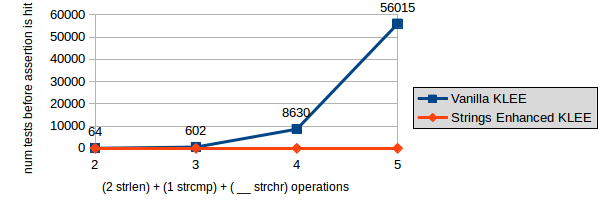
\includegraphics[width=10.0cm]{VanillaKLEE_vs_StringsEnhancedKLEE_num_states.png}\\
\label{Figure_Vanilla_KLEE_State_Explosion}
\end{center}
\end{figure}
%%%%%%%%%%
% Figure %
%%%%%%%%%%
\begin{figure}[htbp]
\begin{center}
  % Requires \usepackage{graphicx}
  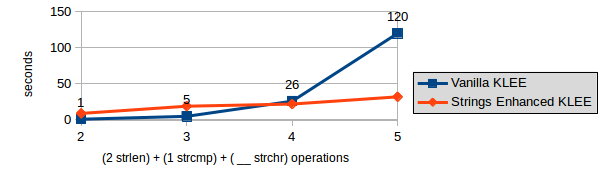
\includegraphics[width=10.0cm]{VanillaKLEE_vs_StringsEnhancedKLEE_time.png}\\
  \caption{Consecutive string library functions cause state explosion.
  \label{Figure_Vanilla_KLEE_time}}
\end{center}
\end{figure}
}

%%%%%%%%%%%%%%%%%%%%%%%%%%%
% SECTION :: Our Approach %
%%%%%%%%%%%%%%%%%%%%%%%%%%%
\section{Our Approach} 
%%%%%%%%%%%%%%%%%%%%%%%%%%%%%%%
% Frame Title :: Our Approach %
%%%%%%%%%%%%%%%%%%%%%%%%%%%%%%%
\frame{\frametitle{Our Approach :: General Description}
%%%%%%%%%%%%%%%%%%
% Items :: Begin %
%%%%%%%%%%%%%%%%%%
\begin{itemize}
\item
When KLEE encounters a string allocation
(on the stack, on the heap or as a constant string)
it will \textbf{physically allocate} that requested memory.
When KLEE updates a string p, during a write operation
like \textbf{p[3]='M'}, it will do so with respect to
the specific memory associated with p.
\item
Our approach uses the notion of \textbf{Abstract Buffers} (AB)
and \textbf{versions}. We do not allocate physical memory
for strings, but rather use string constraints to replace
actual memory allocations and accumulate write changes.
\item
When \textbf{p = malloc(size)} is encountered,
a new (Z3) string sort variable is introduced: AB$_{serial=n,version=0}$,
and a \textbf{length constraint} is added to the state:
(= (str.len AB$_{n,0}$) size).
\item
When \textbf{p[3] = 'M'} is encountered,
an \textbf{additional version} is defined,
and the write operation is expressed as
string constraints between the last 2 versions.
%%%%%%%%%%%%%%%%
% Items :: End %
%%%%%%%%%%%%%%%%
\end{itemize}
}

%%%%%%%%%%%%%%%%%%%%%%%%%%%%%%%%%%%%%%%%
% SECTION :: Augmented Execution State %
%%%%%%%%%%%%%%%%%%%%%%%%%%%%%%%%%%%%%%%%
\section{Our Approach :: In Greater Detail :: Malloc} 
%%%%%%%%%%%%%%%%%%%%%%%%%%%%%%%%%%%%%%%%%%%%
% Frame Title :: Augmented Execution State %
%%%%%%%%%%%%%%%%%%%%%%%%%%%%%%%%%%%%%%%%%%%%
\frame{\frametitle{Our Approach :: In Greater Detail :: Malloc}
%%%%%%%%%%%%%%%%%%
% Items :: Begin %
%%%%%%%%%%%%%%%%%%
\begin{itemize}
\item
KLEE's execution state adds these \textbf{data structures}:
\begin{itemize}
\item
static int numABs = 0;
\item
std::map$<$std::string,int$>$ var2AB;
\item
std::map$<$std::string,ref$<$Expr$>>$ var2ABoffset;
\item
std::map$<$int,ref$<$Expr$>>$ ABSize;
\item
std::map$<$int,int$>$ ABlastVersion;
\end{itemize}
\item
Effect of p = malloc(size) on \textbf{state's data structures}: 
\begin{itemize}
\item
++numABs;
\item
var2AB[p] = numABs;
\item
var2ABoffset[p] = ConstantExpr(0,Expr::Int32);
\item
ABSize[numABs] = size; (size is a ref$<$Expr$>$)
\item
ABlastVersion[numABs] = 0;
\end{itemize}
\item
Effect of p = malloc(size) on \textbf{state's constraints}:
\begin{itemize}
\item
int serialp  = var2AB[p];\\
\item
int versionp = ABlastVersion [serialp];\\
\item
std::string name = makeName(serialp,versionp);
\item
state.addConstraint(StrLengthExpr(StrVarExpr(name)) = size)
\end{itemize}
%%%%%%%%%%%%%%%%
% Items :: End %
%%%%%%%%%%%%%%%%
\end{itemize}
}

%%%%%%%%%%%%%%%%%%%%%%%%%%%%%%%%%%%%%%%%%%%%%%%%%%%%%%%%%%%%%%%%%%%%%
% SECTION :: Our Approach In Greater Detail :: String Modifications %
%%%%%%%%%%%%%%%%%%%%%%%%%%%%%%%%%%%%%%%%%%%%%%%%%%%%%%%%%%%%%%%%%%%%%
\section{Our Approach :: In Greater Detail :: String Modifications} 
%%%%%%%%%%%%%%%%%%%%%%%%%%%%%%%%%%%%%%%%%%%%%%%%%%%%%%%%%%%%%%%%%%%%%%%%%
% Frame Title :: Our Approach In Greater Detail :: String Modifications %
%%%%%%%%%%%%%%%%%%%%%%%%%%%%%%%%%%%%%%%%%%%%%%%%%%%%%%%%%%%%%%%%%%%%%%%%%
\frame{\frametitle{Our Approach :: In Greater Detail :: String Modifications}
%%%%%%%%%%%%%%%%%%
% Items :: Begin %
%%%%%%%%%%%%%%%%%%
\begin{itemize}
\item
Modifying a string with a write operation p[3]='M'
or strcpy(p+offset,q) behave \textit{very similar} in our approach.
\item
Effect of p[3] = 'M' on \textbf{state's data structures}:
\begin{itemize}
\item
ABlastVersion[ var2AB[p] ]++;
\end{itemize}
\item
Effect of p[i]='M' on \textbf{state's constraints}:
\begin{itemize}
\item
(= (str.len AB$_{n,d}$) (str.len AB$_{n,d+1}$))
\item
(= (str.substr AB$_{n,d}$ 0 i-1) (str.substr AB$_{n,d+1}$ 0 i-1))
\item
(= (str.at AB$_{n,d}$ i) (seq.unit c))
\item
(= (str.substr AB$_{n,d}$ i+1 n-i) (str.substr AB$_{n,d+1}$ i+1 n-i))
\end{itemize}
\item
What if p[i]='M' writes outside allocated buffer? (next slide)
%%%%%%%%%%%%%%%%
% Items :: End %
%%%%%%%%%%%%%%%%
\end{itemize}
}

%%%%%%%%%%%%%%%%%%%%%%%%%%%%%%%%%%%%%%%%%%%%%%%%%%%%%%%%%%%%%%%%%%%%%%%%%
% Frame Title :: Our Approach In Greater Detail :: String Modifications %
%%%%%%%%%%%%%%%%%%%%%%%%%%%%%%%%%%%%%%%%%%%%%%%%%%%%%%%%%%%%%%%%%%%%%%%%%
\frame{\frametitle{Our Approach :: In Greater Detail :: String Modifications}
%%%%%%%%%%
% Figure %
%%%%%%%%%%
\begin{figure}[htbp]
\begin{center}
  % Requires \usepackage{graphicx}
  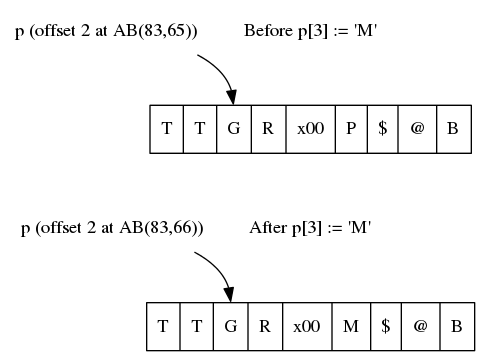
\includegraphics[width=8.0cm]{painting_01.png}
\caption{Writes are expressed as 4 string constraints between
last and second to last versions of the abstract buffer:
equal length, equal content before and after the write,
and the modification itself.
\label{Figure_Expressing_Writes_As_String_Scontstraints}}
\end{center}
\end{figure}
}
%%%%%%%%%%%%%%%%%%%%%%%%%%%%%%%%%%%%%%%%%%%%%%%%%%%%%%%%%%%%%%%%%%
% SECTION :: Our Approach In Greater Detail :: Access Violations %
%%%%%%%%%%%%%%%%%%%%%%%%%%%%%%%%%%%%%%%%%%%%%%%%%%%%%%%%%%%%%%%%%%
\section{Our Approach :: In Greater Detail :: Access Violations} 
%%%%%%%%%%%%%%%%%%%%%%%%%%%%%%%%%%%%%%%%%%%%%%%%%%%%%%%%%%%%%%%%%%%%%%
% Frame Title :: Our Approach In Greater Detail :: Access Violations %
%%%%%%%%%%%%%%%%%%%%%%%%%%%%%%%%%%%%%%%%%%%%%%%%%%%%%%%%%%%%%%%%%%%%%%
\frame{\frametitle{Our Approach :: In Greater Detail :: Access Violations}
%%%%%%%%%%%%%%%%%%
% Items :: Begin %
%%%%%%%%%%%%%%%%%%
\begin{itemize}
\item
The majority of buffer overflows occur in strings,
so we obviously need to model that behaviour, and
detect out of bounds reads and writes like vanilla KLEE does.
\item
Z3 semantics for out of bound string access does \textit{not}
always match our purpose, for example:\\
(= 3 (str.len (str.substring s /*from*/6 /*length*/3)))\\
is \textit{not} true when s has length $\leq$ 5. 
\item
We need to wrap every string action in an ITE Z3 expression(s),
to make sure strings are not written (read) beyond their bounds.
Note that these ITE's can range from simple ones for p[i] := 'M',
to more complex ones needed to model strcmp(p,q), strchr(p,'M') etc.
%%%%%%%%%%%%%%%%
% Items :: End %
%%%%%%%%%%%%%%%%
\end{itemize}
}

%%%%%%%%%%%%%%%%%%%%%%%%%%%%%%%%%%%%%%%%%%%%%%%%%%%%%%%%%%%%%%%%%%
% SECTION :: Our Approach In Greater Detail :: Access Violations %
%%%%%%%%%%%%%%%%%%%%%%%%%%%%%%%%%%%%%%%%%%%%%%%%%%%%%%%%%%%%%%%%%%
\section{Our Approach :: Context Aware Z3 Sorts} 
%%%%%%%%%%%%%%%%%%%%%%%%%%%%%%%%%%%%%%%%%%%%%%%%%%%%%%%%%%%%%%%%%%%%%%
% Frame Title :: Our Approach In Greater Detail :: Access Violations %
%%%%%%%%%%%%%%%%%%%%%%%%%%%%%%%%%%%%%%%%%%%%%%%%%%%%%%%%%%%%%%%%%%%%%%
\frame{\frametitle{Our Approach :: Context Aware Z3 Sorts}
%%%%%%%%%%%%%%%%%%
% Items :: Begin %
%%%%%%%%%%%%%%%%%%
\begin{itemize}
\item
Currently KLEE only supports bit vectors,
so adding a string sort is clearly the first step.
Since string theory interfaces with integers
rather than bit vectors, failing to add an integer sort support
will surely result in bit blasting sort conversions.
\item
To minimize the need for sort conversions,
we came up with the concept of \textbf{context aware Z3 sorts}.
\item
Recall the running example in
[\href{https://arxiv.org/pdf/1605.09446.pdf}{Vijay et al.}] 
where strlen's result was an overflowing bit vector 16. And compare it to the
example in the next slide where strlen can be safely handled
as being an integer
%%%%%%%%%%%%%%%%
% Items :: End %
%%%%%%%%%%%%%%%%
\end{itemize}
}

%%%%%%%%%%%%%%%%%%%%%%%%%%%%%%%%%%%%%%%%%%%%%%%%%%%%%%%%%%%%%%%%%%
% Frame Title :: Character Variable :: Example As Z3 String Sort %
%%%%%%%%%%%%%%%%%%%%%%%%%%%%%%%%%%%%%%%%%%%%%%%%%%%%%%%%%%%%%%%%%%
\frame{\frametitle{Int Variable :: Example As Z3 Int Sort}
%%%%%%%%%%
% Figure %
%%%%%%%%%%
\begin{figure}[htbp]
\begin{center}
  % Requires \usepackage{graphicx}
  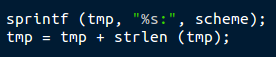
\includegraphics[width=8.0cm]{IntSortForIntVariable.png}
\label{Figure_Char_Variable_As_String_Sort}
\end{center}
\end{figure}
%%%%%%%%%%
% Figure %
%%%%%%%%%%
\begin{figure}[htbp]
\begin{center}
  % Requires \usepackage{graphicx}
  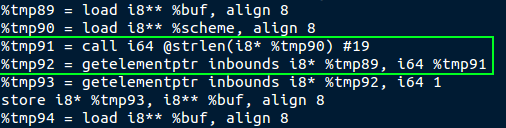
\includegraphics[width=8.0cm]{IntSortForIntVariableLLVMCode.png}
\caption{int's can have integer sort whenever appropriate.
In this example, using an integer as offset inside a buffer
is safe.
\label{Figure_Char_Variable_As_String_Sort_In_LLVM_Code}}
\end{center}
\end{figure}
}


%%%%%%%%%%%%%%%%%%%%%%%%%%%%%%%%%%%%%%%%%%%%%%%%%%%%%%%%%%%%%%%%%%
% Frame Title :: Character Variable :: Example As Z3 String Sort %
%%%%%%%%%%%%%%%%%%%%%%%%%%%%%%%%%%%%%%%%%%%%%%%%%%%%%%%%%%%%%%%%%%
\frame{\frametitle{Character Variable :: Example As Z3 String Sort}
%%%%%%%%%%
% Figure %
%%%%%%%%%%
\begin{figure}[htbp]
\begin{center}
  % Requires \usepackage{graphicx}
  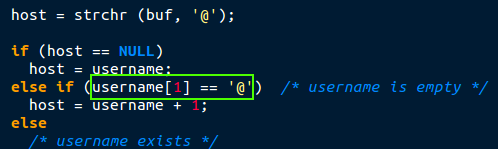
\includegraphics[width=8.0cm]{StringSortForCharVariable.png}
\label{Figure_Char_Variable_As_String_Sort}
\end{center}
\end{figure}
%%%%%%%%%%
% Figure %
%%%%%%%%%%
\begin{figure}[htbp]
\begin{center}
  % Requires \usepackage{graphicx}
  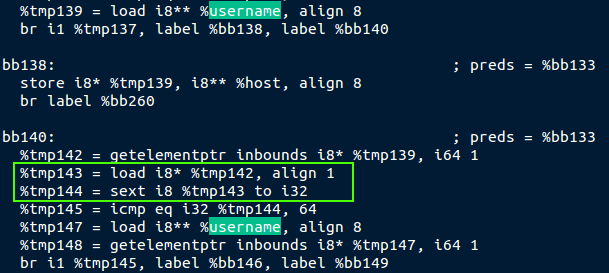
\includegraphics[width=8.0cm]{StringSortForCharVariableLLVMCode.png}
\caption{Characters can have (length 1) string sort whenever appropriate.
In this example tmp144 can be string compared to ``@"
\label{Figure_Char_Variable_As_String_Sort_In_LLVM_Code}}
\end{center}
\end{figure}
}

%%%%%%%%%%%%%%%%%%%%%%%%%%%%%%%%%%%%%%%%%%%%%%%%%%%%%%%%%%%%%%%%%%%
% Frame Title :: Character Variable :: Example As Z3 BitVec8 Sort %
%%%%%%%%%%%%%%%%%%%%%%%%%%%%%%%%%%%%%%%%%%%%%%%%%%%%%%%%%%%%%%%%%%%
\frame{\frametitle{Character Variable :: Example As Z3 BitVec8 Sort}
%%%%%%%%%%
% Figure %
%%%%%%%%%%
\begin{figure}[htbp]
\begin{center}
  % Requires \usepackage{graphicx}
  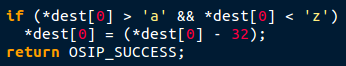
\includegraphics[width=8.0cm]{BitVec8SortForCharVariable.png}
\label{Figure_Char_Variable_As_String_Sort}
\end{center}
\end{figure}
%%%%%%%%%%
% Figure %
%%%%%%%%%%
\begin{figure}[htbp]
\begin{center}
  % Requires \usepackage{graphicx}
  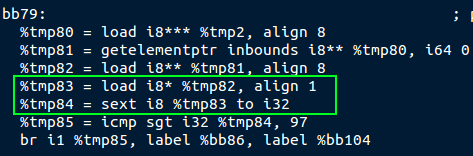
\includegraphics[width=8.0cm]{BitVec8SortForCharVariableLLVMCode.png}
\caption{Characters can have BitVec8 sort whenever appropriate.
In this example tmp84 is sign compared to 'a'
\label{Figure_Char_Variable_As_String_Sort_In_LLVM_Code}}
\end{center}
\end{figure}
}

%%%%%%%%%%%%%%%%%%%%%%%%%%%%%%%%%%
% SECTION :: Real Life Chalenges %
%%%%%%%%%%%%%%%%%%%%%%%%%%%%%%%%%%
\section{Real Life Challenges} 
%%%%%%%%%%%%%%%%%%%%%%%%%%%%%%%%%%%%
% Frame Title :: Real Life Example %
%%%%%%%%%%%%%%%%%%%%%%%%%%%%%%%%%%%%
\frame{\frametitle{Real Life Chalenges
(\href{https://www.cvedetails.com/cve/CVE-2016-10326/}{oSIP2 CVE})}
%%%%%%%%%%%%%%%%%%
% Items :: Begin %
%%%%%%%%%%%%%%%%%%
\begin{itemize}
\item
A heap buffer overflow caused by a malformed SIP message of size 631 bytes
with net payload size = 51+72 bytes. KLEE vanilla fails to find this bug
after $>$ 5 hours of running on server
(though during that time it \textit{did} find another less severe
out of bound read access bug)
\item
Software packages often wrap library functions
which require some find-and-replace human effort.
\item
Software packages sometimes re-write library functions
with slight changes (libosip-strappend uses memmove, for example)
%%%%%%%%%%%%%%%%
% Items :: End %
%%%%%%%%%%%%%%%%
\end{itemize}
}

\end{document}
